\subsection{Melihat Barang yang Didaftarkan}
Halaman ini hanya dapat diakses oleh pengguna yang sudah terdaftar dan sudah login ke dalam sistem. Halaman ini berisi daftar barang yang pernah didaftarkan pengguna, sesuai dengan spesifikasi kasus penggunaan \ref{uc03.03}.\\
\indent Tidak ada \textit{view logic} ataupun logika \textit{UI} khusus dalam halaman ini. Kode sumber implementasi \textit{back-end} dapat dilihat pada kode sumber \ref{cdbe.03-03}.

\begin{lstlisting}[label=cdbe.03-03,style=php,caption=Kode Sumber \textit{Back-end} Melihat Barang yang Pernah Didaftarkan]
/*	
	file : app/Http/Controllers/ItemController
	terkait dengan ItemRepository
*/
 public function index(){
	 /*	method : GET */
	
    $data['items'] = $this->itemRep->getUserItem();
    return view('pages.'.$this->pageFolder.'.index',$data);
}

/*	file : app/Http/Controllers/ItemRepository */
public function getUserItem()
{
    return Auth::user()->item()->orderBy('end_time','desc')->get();
}
\end{lstlisting}

\begin{figure}[H]
	\centering
	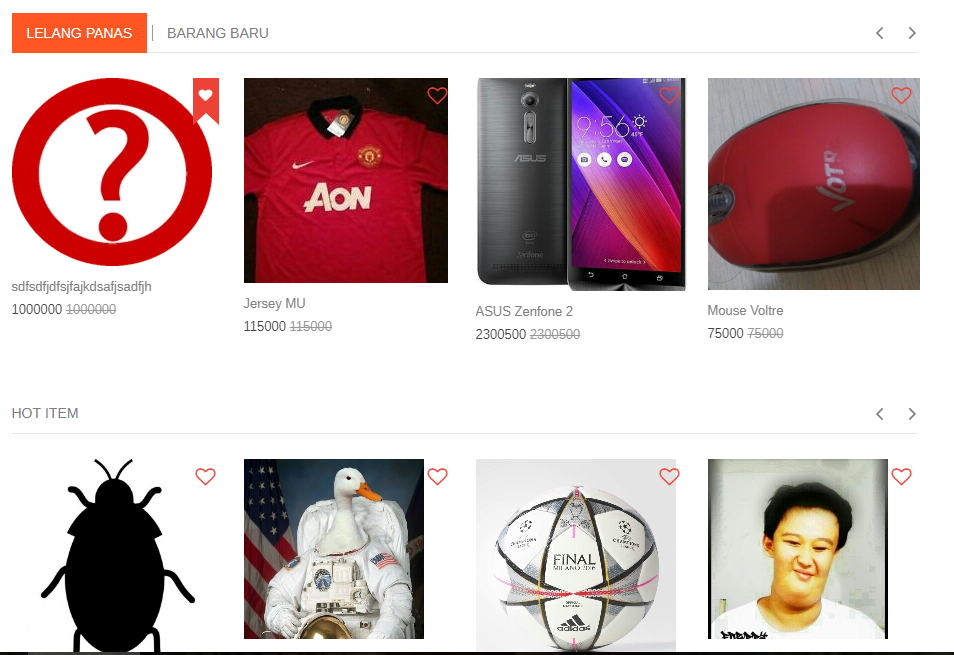
\includegraphics[width=\textwidth]{images/bab4/ui/02-01.png}
	\caption{Halaman antarmuka }
	\label{ui.02-01}
\end{figure}

